%!TEX root = ../thesis.tex
%*******************************************************************************
%****************************** Third Chapter **********************************
%*******************************************************************************
\chapter{Planificación y estado de avance.}

% **************************** Define Graphics Path **************************
\ifpdf
    \graphicspath{{Chapter5/Figs/Raster/}{Chapter5/Figs/PDF/}{Chapter5/Figs/}}
\else
    \graphicspath{{Chapter5/Figs/Vector/}{Chapter5/Figs/}}
\fi

Es posible pensar en este proyecto de Tesis, como un conjunto de postulaciones y planteamientos de nuevas metodologías basadas en el uso de técnicas de minería de datos que permitan estudiar mutaciones en conjuntos de datos y que culminan con una gran temática, que aborda la implementación de una herramienta computacional para el diseño de mutaciones.

Dado esto, el proyecto en sí, puede dividirse en tres grandes objetivos, de los cuales, los conocimientos y destrezas adquiridas en los primeros dos, son necesarias para cumplir con el tercer gran objetivo. Esto, es posible observarlo en la Figura \ref{cap5:fig1}.

\begin{figure}[!h]
	
	\centering
	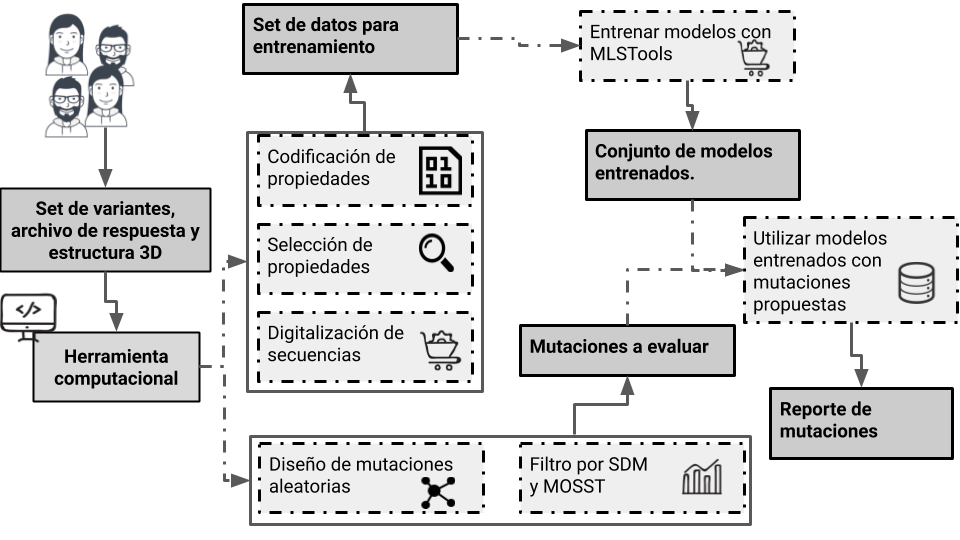
\includegraphics[scale=.5]{fig1.png}
	\caption{Esquema representativo de objetivos generales involucrados en el desarrollo del proyecto.}
	\label{cap5:fig1}
\end{figure}

El primer objetivo, se basa en la construcción de modelos de clasificación o regresión basados en algoritmos de aprendizaje supervisado, enfocados en el estudio de mutaciones puntuales en una proteína y cómo afectan éstas en términos de una respuesta conocida, como por ejemplo, estabilidad, productividad, actividad, etc. Esto, va en directo beneficio del estudio de nuevas mutantes o variantes en proteínas de interés, apoyados en una metodología que maximiza el desempeño de los modelos y sin incurrir en costos computacionales elevados. No obstante, el hecho de manipular nuevas mutaciones, requiere una verificación experimental. Sin embargo, esto permite minimizar los costos económicos y de recursos humanos que conlleva estudiar un gran conjunto de espacios muestrales de mutaciones. 

Por otro lado, el segundo objetivo se basa principalmente en representar secuencias lineales de proteínas a partir de la digitalización de propiedades fisicoquímicas y empleando transformadas de Fourier como representación de espectros de frecuencias. Si bien, el enfoque principal es la representación en sí, el objetivo también abarca el cómo utilizar estas representaciones para el entrenamiento de modelos de clasificación/regresión o el reconocimiento de patrones e identificación de residuos que aportan a las propiedades fisicoquímicas.

Finalmente, el tercer gran objetivo, comprende el desarrollo de una herramienta computacional, basada en técnicas de minería de datos para el diseño de mutaciones en proteínas de interés. El cómo se abarcará esta problemática, comprende, por un lado, definir representaciones de las secuencias lineales y cómo codificar sus propiedades fisicoquímicas, en conjunto, con el entrenamiento de modelos de clasificación/regresión que permitan evaluar nuevas mutantes. Es decir, los enfoques propuestos en los capítulos \ref{cap3} y \ref{cap2}, respectivamente. Demostrando así, las relaciones existentes entre cada capítulo y cómo estos apuntan a un objetivo general que conlleva aplicar minería de datos en el estudio de mutaciones puntuales asociados a la ingeniería de proteínas.

Con el fin de trazar los panoramas asociados al desarrollo de cada metodología y exponer el estado de avance del proyecto en cuanto a las diferentes actividades desarrolladas, en el presente capítulo, se expone un conjunto de actividades resumen de cada objetivo, asociados a un tiempo estimativo que conlleva el cumplimiento de estos y a su vez, las tareas ya han sido desarrolladas, junto con las actividades pendientes a realizar.

\section{Planificación}

La planificación se centra en cumplir los tres grandes objetivos y se plantea una estimación del tiempo que conlleva el desarrollo de cada una de las temáticas. Se exponen diferentes tareas generales que aportan a cumplir los objetivos y el tiempo estimativo, considerando un desarrollo general de 3 años como máximo para todas las actividades planteadas. Es importante mencionar y recalcar que este itinerario es un estimativo y sólo se exponen las tareas principales para el desarrollo del proyecto.

En las Tablas \ref{tab:obj1}, \ref{tab:obj2}  y \ref{tab:obj3} se exponen las actividades relacionadas al objetivo principal que aportan a cumplir, además del tiempo estimativo de desarrollo.

% Please add the following required packages to your document preamble:
% \usepackage{longtable}
% Note: It may be necessary to compile the document several times to get a multi-page table to line up properly
\begin{longtable}[c]{l|l|l|}
	\hline
	\multicolumn{3}{|c|}{\textbf{Resumen de actividades enfocadas en el desarrollo de modelos de clasificación}} \\ \hline
	\endfirsthead
	%
	\endhead
	%
	\multicolumn{1}{|c|}{\textbf{\#}} & \multicolumn{1}{c|}{\textbf{Actividad a desarrollar}} & \multicolumn{1}{c|}{\textbf{\begin{tabular}[c]{@{}c@{}}Tiempo\\ (semanas)\end{tabular}}} \\ \hline
	\multicolumn{1}{|l|}{1.} & Búsqueda de mutaciones en bases de datos y reportes publicados & 3 \\ \hline
	\multicolumn{1}{|l|}{2.} & Preparación y análisis del conjunto de datos a estudiar & 3 \\ \hline
	\multicolumn{1}{|l|}{3.} & Describir set de datos enfocados en propiedades termodinámicas & 5 \\ \hline
	\multicolumn{1}{|l|}{4.} & Describir set de datos enfocados en conceptos filogenéticos &  5\\ \hline
	\multicolumn{1}{|l|}{5.} & Implementar algoritmos de aprendizaje supervisado & 3 \\ \hline
	\multicolumn{1}{|l|}{6.} & Implementar metodología propuesta & 2 \\ \hline
	\multicolumn{1}{|l|}{7.} & \begin{tabular}[c]{@{}l@{}}Entrenar modelos de clasificación/regresión para conjuntos de\\ proteínas seleccionados\end{tabular} & 5 \\ \hline
	\multicolumn{1}{|l|}{8.} & Revisar resultados y reportar conclusiones & 5 \\ \hline
	\multicolumn{1}{|l|}{9.} & Implementar herramienta computacional asociada & 5 \\ \hline
	\multicolumn{1}{|l|}{10.} & Testear y generar depuración de herramienta & 3 \\ \hline
	& \multicolumn{1}{c|}{\textbf{Total Semanas}} & \multicolumn{1}{c|}{\textbf{39}} \\ \cline{2-3} 
	\caption{Resumen de actividades principales a desarrollar, enfocadas el desarrollo de modelos predictivos para mutaciones puntuales en proteínas.}
	\label{tab:obj1}\\
\end{longtable}


% Please add the following required packages to your document preamble:
% \usepackage{longtable}
% Note: It may be necessary to compile the document several times to get a multi-page table to line up properly
\begin{longtable}[c]{l|l|l|}
	\hline
	\multicolumn{3}{|c|}{\textbf{Resumen de actividades enfocadas en la codificación de secuencias lineales}} \\ \hline
	\endfirsthead
	%
	\endhead
	%
	\multicolumn{1}{|c|}{\textbf{\#}} & \multicolumn{1}{c|}{\textbf{Actividad a desarrollar}} & \multicolumn{1}{c|}{\textbf{\begin{tabular}[c]{@{}c@{}}Tiempo\\ (semanas)\end{tabular}}} \\ \hline
	\multicolumn{1}{|l|}{1.} & Búsqueda de secuencias lineales & 2 \\ \hline
	\multicolumn{1}{|l|}{2.} & Búsqueda de conjuntos de datos reportados con respuesta conocida & 2 \\ \hline
	\multicolumn{1}{|l|}{3.} & Codificación de secuencias lineales empleando propiedades descritas en AAindex & 3 \\ \hline
	\multicolumn{1}{|l|}{4.} & Selección de propiedades informativas y generación de propiedades consenso & 4 \\ \hline
	\multicolumn{1}{|l|}{5.} & Digitalización de propiedades fisicoquímicas empleando transformadas de Fourier & 4 \\ \hline
	\multicolumn{1}{|l|}{6.} & Identificación de residuos relevantes para la propiedad fisicoquímica & 3 \\ \hline
	\multicolumn{1}{|l|}{7.} & \begin{tabular}[c]{@{}l@{}}Aplicación de métodos de clustering para búsqueda de patrones en espectros de\\ frecuencia\end{tabular} & 4 \\ \hline
	\multicolumn{1}{|l|}{8.} & \begin{tabular}[c]{@{}l@{}}Entrenamiento de modelos de clasificación/regresión con descriptores basados en\\ espectros de frecuencia\end{tabular} & 4 \\ \hline
	\multicolumn{1}{|l|}{9.} & Revisar resultados y reportar conclusiones & 5 \\ \hline
	\multicolumn{1}{|l|}{10.} & Implementar herramienta computacional asociada & 5 \\ \hline
	\multicolumn{1}{|l|}{11.} & Testear y generar depuración de herramienta & 3 \\ \hline
	& \multicolumn{1}{c|}{\textbf{Total Semanas}} & \multicolumn{1}{c|}{\textbf{39}} \\ \cline{2-3} 
	\caption{Resumen de actividades asociadas a la codificación y digitalización de propiedades fisicoquímicas}
	\label{tab:obj2}\\
\end{longtable}

% Please add the following required packages to your document preamble:
% \usepackage{longtable}
% Note: It may be necessary to compile the document several times to get a multi-page table to line up properly
\begin{longtable}[c]{l|l|l|}
	\hline
	\multicolumn{3}{|c|}{\textbf{\begin{tabular}[c]{@{}c@{}}Resumen de actividades enfocadas en implementación de \\ herramienta para diseño de mutaciones\end{tabular}}} \\ \hline
	\endfirsthead
	%
	\endhead
	%
	\multicolumn{1}{|c|}{\textbf{\#}} & \multicolumn{1}{c|}{\textbf{Actividad a desarrollar}} & \multicolumn{1}{c|}{\textbf{\begin{tabular}[c]{@{}c@{}}Tiempo\\ (semanas)\end{tabular}}} \\ \hline
	\multicolumn{1}{|l|}{1.} & Implementación módulo codificación de secuencias lineales & 3 \\ \hline
	\multicolumn{1}{|l|}{2.} & Implementación módulo selección de propiedades & 3 \\ \hline
	\multicolumn{1}{|l|}{3.} & Implementación módulo digitalización de propiedades & 3 \\ \hline
	\multicolumn{1}{|l|}{4.} & Implementación módulo entrenamiento de modelos & 4 \\ \hline
	\multicolumn{1}{|l|}{5.} & Implementación servicio API MOSST & 4 \\ \hline
	\multicolumn{1}{|l|}{6.} & Implementación servicio API SDM & 4 \\ \hline
	\multicolumn{1}{|l|}{7.} & Implementación servicio propuesta de mutaciones & 5 \\ \hline
	\multicolumn{1}{|l|}{8.} & Implementación servicio gestor de sistema de colas & 4 \\ \hline
	\multicolumn{1}{|l|}{9.} & Implementación controlador de solicitudes & 7 \\ \hline
	\multicolumn{1}{|l|}{10.} & Implementación de servicio creación de jobs en Front-end & 5 \\ \hline
	\multicolumn{1}{|l|}{11.} & Implementación de servicio búsqueda de jobs & 2 \\ \hline
	\multicolumn{1}{|l|}{12.} & Implementación de servicio visualización de resultados & 10 \\ \hline
	\multicolumn{1}{|l|}{13.} & Implementación visualización de mutaciones propuestas & 6 \\ \hline
	\multicolumn{1}{|l|}{14.} & Implementación servicio de notificaciones & 2 \\ \hline
	\multicolumn{1}{|l|}{15.} & Teste y debug herramienta computacional & 5 \\ \hline
	& \multicolumn{1}{c|}{\textbf{Total Semanas}} & \multicolumn{1}{c|}{\textbf{79}} \\ \cline{2-3} 
	\caption{Resumen de actividades asociadas al desarrollo de herramienta computacional web para diseño de mutaciones}
	\label{tab:obj3}\\
\end{longtable}

Para el desarrollo del primer objetivo, se contempla un total de 39 semanas, de la misma forma que para el objetivo 2, mientras que para el objetivo 3, se contempla un total de 79 semanas. En total se estima un total de 3 años, para poder cumplir con los objetivos planteados, tiempo en el cual, se piensa desarrollar las actividades propuestas previamente. 

Un punto importante a destacar, es que en sí, cada objetivo consta del desarrollo de una herramienta en particular, enfocada en el objetivo en sí, con el enfoque principal de brindar un apoyo sustancial a investigadores asociados al estudio de mutaciones e involucrados en ingeniería de proteínas.

\section{Estado de avance}

Con respecto al estado de avance, actualmente se tiene desarrollado un porcentaje significativo de lo planteado en el capítulo 1, al menos, en cuanto a desarrollo de módulos, implementación de código fuente y búsqueda de set de datos y conjuntos de proteínas a evaluar.

A modo resumen, se expone una variación de la Tabla \ref{tab:obj1}, adicionando el avance en el que se encuentra dicho desarrollo en términos de porcentaje, la cual se observa en la Tabla \ref{tab:obj4}.


% Please add the following required packages to your document preamble:
% \usepackage{longtable}
% Note: It may be necessary to compile the document several times to get a multi-page table to line up properly
\begin{longtable}[c]{l|l|l|l|}
	\hline
	\multicolumn{4}{|c|}{\textbf{Resumen de actividades enfocadas en el desarrollo de modelos de clasificación}} \\ \hline
	\endfirsthead
	%
	\endhead
	%
	\multicolumn{1}{|c|}{\textbf{\#}} & \multicolumn{1}{c|}{\textbf{Actividad a desarrollar}} & \multicolumn{1}{c|}{\textbf{\begin{tabular}[c]{@{}c@{}}Tiempo\\ (semanas)\end{tabular}}} & \multicolumn{1}{c|}{\textbf{\begin{tabular}[c]{@{}c@{}}Estado\\ Avance\end{tabular}}} \\ \hline
	\multicolumn{1}{|l|}{1.} & \begin{tabular}[c]{@{}l@{}}Búsqueda de mutaciones en bases de datos y\\ reportes publicados\end{tabular} & 3 & 100\% \\ \hline
	\multicolumn{1}{|l|}{2.} & Preparación y análisis del conjunto de datos a estudiar & 3 & 100\% \\ \hline
	\multicolumn{1}{|l|}{3.} & \begin{tabular}[c]{@{}l@{}}Describir set de datos enfocados en propiedades\\ termodinámicas\end{tabular} & 5 & 100\% \\ \hline
	\multicolumn{1}{|l|}{4.} & Describir set de datos enfocados en conceptos filogenéticos & 5 & 0\% \\ \hline
	\multicolumn{1}{|l|}{5.} & Implementar algoritmos de aprendizaje supervisado & 3 & 100\% \\ \hline
	\multicolumn{1}{|l|}{6.} & Implementar metodología propuesta & 2 & 50\% \\ \hline
	\multicolumn{1}{|l|}{7.} & \begin{tabular}[c]{@{}l@{}}Entrenar modelos de clasificación/regresión para\\ conjuntos de proteínas seleccionados\end{tabular} & 5 & 0\% \\ \hline
	\multicolumn{1}{|l|}{8.} & Revisar resultados y reportar conclusiones & 5 & 0\% \\ \hline
	\multicolumn{1}{|l|}{9.} & Implementar herramienta computacional asociada & 5 & 0\% \\ \hline
	\multicolumn{1}{|l|}{10.} & Testear y generar depuración de herramienta & 3 & 0\% \\ \hline
	& \multicolumn{1}{c|}{\textbf{Total Semanas}} & \multicolumn{1}{c|}{\textbf{39}} & \textbf{38\%} \\ \cline{2-4} 
	\caption{Resumen y estado de actividades principales asociadas al desarrollo de modelos de clasificación en mutaciones puntuales.}
	\label{tab:obj4}\\
\end{longtable}

Se puede apreciar, que se ha completado cerca del 40\% del trabajo asociado al desarrollo de modelos de predictivos, siendo tareas pendientes, caracterizar mutaciones desde puntos de vista filogenéticos, el entrenamiento de modelos y el desarrollo de una herramienta computacional asociada al entrenamiento de conjuntos de datos para predecir respuestas conocidas.

Finalmente, tanto la planificación como el estado de avance expuesto, se muestran con el fin de denotar la factibilidad del proyecto y cuáles son las actividades que se tienen consideradas en cada etapa de desarrollo. Como se mencionó previamente, el trabajo de tesis, se plantea como un conjunto de metodologías e implementación de herramientas computacionales, que permitan el estudio de las mutaciones y sirva de apoyo en el área de ingeniería de proteínas, culminando con el ambicioso objetivo de generar una herramienta que permita el diseño de mutantes, siendo ésta la gran premisa de este proyecto de tesis.